\chapter{Appendix2: Kerberos}
\label{appendix:kerberos}
This appendix describes in detail the Kerberos authentication flow. This flow is depicted in Figure \ref{fig:kerberos}.

\begin{figure}[!ht]
	\centering
	\caption{Kerberos authentication flow}
	\label{fig:kerberos}
	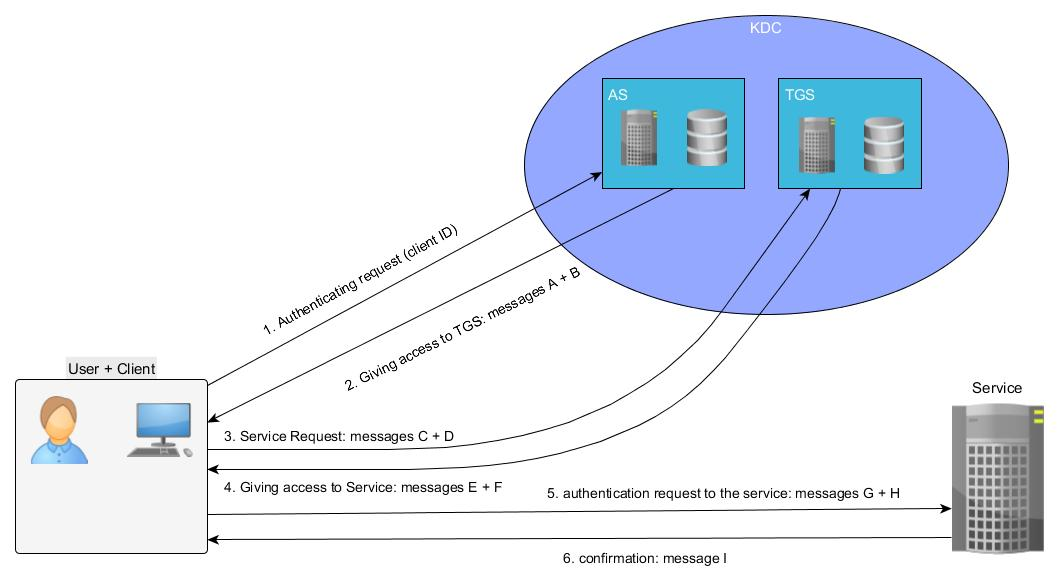
\includegraphics[scale=0.4]{images/kerberos}
\end{figure}

\begin{enumerate}
	\item The user first authenticate with the Authentication Server. This step consists only in sending the user ID in clear text (it is assumed that the user is already registered, and that the AS knows the keys of all its users).
	\item The AS checks if it knows the user. If yes, it sends two messages back: 
	\begin{enumerate}[label=\bfseries\Alph*)]
		\item client TGS session key $k_{TGS/user}$ encrypted with $k_{user}$;
		\item $TGT$ (Ticket Granting Ticket), which allows the client to contact the TGS. It contains the predefined TGS session key  $k_{TGS/user}$, along with the client ID, the client network address, the validity time of the ticket, etc. The $TGT$ is encrypted with $k_{TGS}$ so that only the TGS can decrypt it.
	\end{enumerate}
	The client can decrypt A but not B, since it doesn't know $k_{TGS}$. From what it now has, the client can request services access.
	
	\item The client requests a specific service, by sending the two following messages:
	\begin{enumerate}[label=\bfseries\Alph*), resume]
		\item $\lbrace TGT, service ID \rbrace$
		\item $Authenticator=\lbrace client ID, timestamp \rbrace$ encrypted with $k_{TGS/user}$ 
	\end{enumerate}
	Once again, only the TGS can decrypt both of the messages.
	
	\item When receiving message \textbf{C} and \textbf{D}, the TGS verify that the ticket $TGT$ is valid and decrypt the $Authenticator$ with the session key of the user. It is assumed here that every services are formerly registered to the TGS, so that the TGS has the key of the required service. If it has it, it then sends the two following messages:
	\begin{enumerate}[label=\bfseries\Alph*), resume]
		\item Client / SS session key $k_{SS/user}$ encrypted with $k_{TGS/user}$.
		\item Client to AS Ticket, containing information aimed at the server ($k_{SS/user}$, validity period, user ID, user address, etc). It is encrypted with $k_{SS}$ so that only the Service Server can decrypt it.
	\end{enumerate}
	
	\item The client know has enough information to connect to the SS, with the two following messages:
	\begin{enumerate}[label=\bfseries\Alph*), resume]
		\item same as H.
		\item New $Authenticator$ containing the client ID, a new timestamp, encrypted with $k_{SS/user}$.
	\end{enumerate}
	
	\item When the Service Server receives both messages, it can decrypt the session key, and confirm its true identity with a last message
	\begin{enumerate}[label=\bfseries\Alph*), resume]
		\item The timestamp found in message H + 1, encrypted with the session key.
	\end{enumerate}
\end{enumerate}